\chapter{canonical quantization}
\begin{itemize}
	\item A. Zee: the canonical and the path integral formalisms often appear complementary, in the sense that results difficult to see in one are clear in the other.
	
	\item \textbf{nobody is perfect:}
	\begin{itemize}
		\item \textbf{canonical quantization:} 如何定义场算符乘积的顺序.
		
		\item \textbf{path integral:} integration measure.
	\end{itemize}
\end{itemize}

\section{Heisenberg and Dirac}
\subsection{quantum mechanics}
\begin{itemize}
	\item 单粒子的 classical Lagrangian 为
	\begin{equation}
		L = \frac{1}{2} \dot{q}^2 - V(q) \Longrightarrow \begin{dcases}
			p = \dot{q} \\
			H = p \dot{q} - L = \frac{1}{2} p^2 + V(q)
		\end{dcases}.
	\end{equation}
	
	\item canonical commutation relation 如下,
	\begin{equation}
		[p, q] = - i,
	\end{equation}
	因此, 算符的演化方程为
	\begin{equation}
		\begin{dcases}
			\frac{d p}{dt} = i [H, p] = - V'(q) \\
			\frac{d q}{dt} = i [H, q] = p
		\end{dcases}.
	\end{equation}
	
	\begin{tcolorbox}[title=calculation:]
		\begin{equation}
			\begin{dcases}
				[p, q] = - i \\
				[p, q^2] = - 2 i q \\
				\multicolumn{1}{c}{\vdots} \\
				[p, q^n] = - i q^{n - 1} + q [p, q^{n - 1}]
			\end{dcases} \Longrightarrow [p, q^n] = - i n q^{n - 1} \Longrightarrow [p, V(q)] = - i V'(q).
		\end{equation}
	\end{tcolorbox}
	
	\noindent\rule[0.5ex]{\linewidth}{0.5pt} % horizontal line
	
	\item follow Dirac's approach,
	\begin{equation}
		a = \frac{1}{\sqrt{2 \omega}} (\omega q + i p) \iff \begin{dcases}
			q = \frac{1}{\sqrt{2 \omega}} (a + a^\dag) \\
			p = - i \sqrt{\frac{\omega}{2}} (a - a^\dag)
		\end{dcases} \Longrightarrow [a, a^\dag] = 1,
	\end{equation}
	算符 $a$ 的演化方程为
	\begin{equation}
		\frac{d a}{dt} = - i \sqrt{\frac{\omega}{2}} \Big( \frac{1}{\omega} V'(q) + i p \Big).
	\end{equation}
\end{itemize}

\subsection{scalar field}
\begin{itemize}
	\item 标量场的 Lagrangian 为
	\begin{equation}
		L = \int d^D x \, \Big( - \frac{1}{2} ((\partial \phi)^2 + m^2 \phi^2) - u(\phi) \Big),
	\end{equation}
	canonical commutation relation 为
	\begin{equation} \label{canonical quantization.1.8}
		\pi(\vec{x}, t) = \frac{\delta L(t)}{\delta \partial_0 \phi(\vec{x}, t)} = \partial_0 \phi(\vec{x}, t) \quad \text{and} \quad [\pi(\vec{x}, t), \phi(\vec{y}, t)] = - i \delta^{(D)}(\vec{x} - \vec{y}),
	\end{equation}
	标量场的 Hamiltonian 为
	\begin{equation} \label{canonical quantization.1.9}
		H = \int d^D x \, (\pi \phi - \mathcal{L}) = \int d^D x \, \Big( \frac{1}{2} (\pi^2 + |\vec{\nabla} \phi|^2 + m^2 \phi^2) + u(\phi) \Big).
	\end{equation}
	
	\noindent\hdashrule[0.5ex]{\linewidth}{0.5pt}{1mm} % horizontal dashed line
	
	\item 算符的演化方程为
	\begin{equation} \label{canonical quantization.1.10}
		\begin{dcases}
			\partial_0 \phi = i [H, \phi] = \pi \\
			\partial_0 \pi = i [H, \pi] = (- \vec{\nabla}^2 + m^2) \phi + \frac{d u}{d\phi}
		\end{dcases} \Longrightarrow (\partial^2 - m^2) \phi - \frac{d u}{d\phi} = 0.
	\end{equation}
	
	\item 当 $u(\phi) = 0$ 时, 求解场方程 \eqref{canonical quantization.1.10} 和 canonical commutation relation \eqref{canonical quantization.1.8} 得到
	\begin{equation} \label{canonical quantization.1.11}
		\phi(\vec{x}, t) = \int \frac{d^D k}{(2 \pi)^D 2 \omega_k} (\alpha_k(t) e^{i \vec{k} \cdot \vec{x}} + \alpha^\dag_k(t) e^{- i \vec{k} \cdot \vec{x}}),
	\end{equation}
	其中
	\begin{equation}
		\alpha_k(t) = \sqrt{(2 \pi)^D 2 \omega_k} \, a_{\vec{k}} e^{- i \omega_k t} \quad \text{and} \quad [a_{\vec{p}}, a^\dag_{\vec{q}}] = \delta^{(D)}(\vec{p} - \vec{q}).
	\end{equation}
	另外, 在后面的笔记中使用简记 $\sqrt{(2 \pi)^D 2 \omega_k} = \rho(k)$.
	
	\begin{tcolorbox}[title=calculation:]
		求解场方程 \eqref{canonical quantization.1.10}, 得到
		\begin{equation}
			\phi(\vec{x}, t) = \int \frac{d^D k}{(2 \pi)^D} (\alpha_{\vec{k}} e^{i (- \omega_k t + \vec{k} \cdot \vec{x})} + \alpha^\dag_{\vec{k}} e^{- i (- \omega_k t + \vec{k} \cdot \vec{x})}),
		\end{equation}
		代入 canonical commutation relation \eqref{canonical quantization.1.8}, 有 (其中 $x^0 = y^0 = t, k^0 = \omega_k$)
		\begin{align}
			& \int \frac{d^D k_2}{(2 \pi)^D} \Big( - i \omega_{k_1} [\alpha_{\vec{k}_1}, \alpha_{\vec{k}_2}] e^{i (k_1 \cdot x + k_2 \cdot y)} + i \omega_{k_1} [\alpha^\dag_{\vec{k}_1}, \alpha^\dag_{\vec{k}_2}] e^{- i (k_1 \cdot x + k_2 \cdot y)} \notag \\
			& - i \omega_{k_1} [\alpha_{\vec{k}_1}, \alpha^\dag_{\vec{k}_2}] e^{i (k_1 \cdot x - k_2 \cdot y)} + i \omega_{k_1} [\alpha^\dag_{\vec{k}_1}, \alpha_{\vec{k}_2}] e^{- i (k_1 \cdot x - k_2 \cdot y)} \Big) = - i e^{i \vec{k}_1 \cdot (\vec{x} - \vec{y})} \notag \\
			\Longrightarrow & \begin{dcases}
				[\alpha_{\vec{k}_1}, \alpha_{\vec{k}_2}] = \frac{1}{2 \omega_{k_1}} \delta^{(D)}(\vec{k}_1 + \vec{k}_2) \Longrightarrow [\alpha_{\vec{k}}, \alpha_{\vec{k}}] \neq 0 & \text{wrong} \\
				[\alpha_{\vec{k}_1}, \alpha^\dag_{\vec{k}_2}] = \frac{1}{2 \omega_{\vec{k}_1}} \delta^{(D)}(\vec{k}_1 - \vec{k}_2) & \text{right}
			\end{dcases}.
		\end{align}
	\end{tcolorbox}
	
	\item 代入 \eqref{canonical quantization.1.9} 可得 (依然是 $u(\phi) = 0$ 的情况下)
	\begin{equation} \label{canonical quantization.1.15}
		H = \int d^D k \, \omega_k \frac{a^\dag_{\vec{k}} a_{\vec{k}} + a_{\vec{k}} a^\dag_{\vec{k}}}{2} = \int d^D k \, \omega_k \Big( a^\dag_{\vec{k}} a_{\vec{k}} + \frac{1}{2} \delta^{(D)}(0) \Big) \Longrightarrow \braket{0 | H | 0} = V \int \frac{d^D k}{(2 \pi)^D} \frac{1}{2} \omega_k,
	\end{equation}
	其中, $V = \int d^D x = (2 \pi)^D \delta^{(D)}(0)$.
	
	\noindent\rule[0.5ex]{\linewidth}{0.5pt} % horizontal line
	
	\item vacuum state 定义为 $a_{\vec{k}} \ket{0} = 0$, 有
	\begin{equation}
		\braket{0 | \phi(x) \phi(y) | 0} = \int \frac{d^D k}{(2 \pi)^D 2 \omega_k} e^{i k \cdot (x - y)},
	\end{equation}
	其中 $k^0 = \omega_k$. 因此, 对比 \eqref{free field theory.2.1}, 有
	\begin{equation} \label{canonical quantization.1.17}
		\braket{0 | T(\phi(x) \phi(y)) | 0} = i D(x - y).
	\end{equation}
\end{itemize}

\subsubsection{energy-momentum tensor}
\begin{itemize}
	\item scalar field 的动量算符为
	\begin{equation}
		P^\mu = \int d^D x \, T^{0 \mu} = \int d^D k \, k^\mu a^\dag_{\vec{k}} a_{\vec{k}},
	\end{equation}
	其中, energy-momentum tensor 见 subsection \ref{classical field theory and Noether's theorem.2.3}, 另外 $P^0 = H$ 还有一个 vacuum energy.
\end{itemize}

\section{interaction picture}
\begin{itemize}
	\item 注意, 在 $u(\phi) \neq 0$ 的情况下, (即便在 Schrödinger's picture 里, $t = 0$ 时) \eqref{canonical quantization.1.11} 不再成立, 因此无法通过 Schrödinger's picture or Heisenberg's picture 求解存在相互作用的场论.
	
	\item 将 Hamiltonian 分成两个部分,
	\begin{equation}
		H = H_0 + H'.
	\end{equation}
	
	\item operators 以自由场的 Hamiltonian 演化,
	\begin{equation} \label{canonical quantization.2.2}
		O_I(t) = U_0^\dag(t, 0) O(0) U_0(t, 0) \quad \text{where} \quad U_0(t_2, t_1) = \mathrm{Texp} \Big( - i \int_{t_1}^{t_2} dt \, H_0 \Big),
	\end{equation}
	states 以如下方式演化,
	\begin{equation} \label{canonical quantization.2.3}
		\ket{\psi(t)}_I = U_0^\dag(t, 0) U(t, 0) \ket{\psi(0)} \quad \text{where} \quad U(t_2, t_1) = \mathrm{Texp} \Big( - i \int_{t_1}^{t_2} dt \, H \Big),
	\end{equation}
	因此
	\begin{equation}
		\ket{\psi(t_2)}_I = U_I(t_2, t_1) \ket{\psi(t_1)}_I \quad \text{where} \quad U_I(t_2, t_1) = \mathrm{Texp} \Big( - i \int_{t_1}^{t_2} dt \, H_I(t) \Big),
	\end{equation}
	注意, \eqref{canonical quantization.2.2} 和 \eqref{canonical quantization.2.3} 中, $\mathrm{Texp}$ 里的 $H, H_0$ 都是 Schrödinger's picture 里的算符.
	
	\begin{tcolorbox}[title=calculation:]
		首先有
		\begin{equation}
			U_I(t_2, t_1) = U_0^\dag(t_2, 0) U(t_2, t_1) U_0(t_1, 0),
		\end{equation}
		因此
		\begin{align}
			\frac{d}{dt} U_I(t, t_0) &= i H_0 U_I(t, t_0) - i U_0^\dag(t, 0) H U(t, t_0) U_0(t_0, 0) \notag \\
			&= - i \underbrace{U_0^\dag(t, 0) H' U_0(t, 0)}_{= H_I(t)} U_I(t, t_0).
		\end{align}
	\end{tcolorbox}
\end{itemize}

\section{scattering amplitude}
\begin{itemize}
	\item 最一般的过程是 $p_1, \cdots, p_m \rightarrow q_1, \cdots, q_n$, 其 scattering amplitude 为
	\begin{equation}
		\braket{q_1, \cdots, q_n | U_0^\dag(- \infty, 0) U_I(+ \infty, - \infty) U_0(- \infty, 0) | p_1, \cdots, p_m},
	\end{equation}
	一般会忽略掉 $U_0$ 产生的相位.
	
	\noindent\rule[0.5ex]{\linewidth}{0.5pt} % horizontal line
	
	\item 考虑 $\phi^4$ 理论中的 $k_1, k_2 \rightarrow k_3, k_4$ 过程,
	\begin{equation}
		\braket{k_3, k_4 | e^{- i \int d^d x \, \frac{\lambda}{4!} \phi^4} | k_1, k_2},
	\end{equation}
	对 $\lambda$ 展开, 0 阶项为
	\begin{align}
		\text{0th order term} &= \braket{k_3, k_4 | k_1, k_2} \notag \\
		&= \rho(k_1) \rho(k_2) \rho(k_3) \rho(k_4) \braket{0 | a_{\vec{k}_3} a_{\vec{k}_4} a^\dag_{\vec{k}_1} a^\dag_{\vec{k}_2} | 0} \notag \\
		&= \rho(k_1) \rho(k_2) \rho(k_3) \rho(k_4) \Big( \underbrace{\braket{0 | \wick{
			\c1 a_{\vec{k}_3} \c2 a_{\vec{k}_4} \c1 a^\dag_{\vec{k}_1} \c2 a^\dag_{\vec{k}_2}
		} | 0}}_{= \delta^{(D)}_{3 1} \delta^{(D)}_{4 2}} + \underbrace{\braket{0 | \wick{
			\c1 a_{\vec{k}_3} \c2 a_{\vec{k}_4} \c2 a^\dag_{\vec{k}_1} \c1 a^\dag_{\vec{k}_2}
		} | 0}}_{= \delta^{(D)}_{3 2} \delta^{(D)}_{4 1}} \Big) \notag \\
		&= (2 \pi)^{2 D} 4 \omega_{k_1} \omega_{k_2} (\delta^{(D)}(\vec{k}_1 - \vec{k}_3) \delta^{(D)}(\vec{k}_2 - \vec{k}_4) + \delta^{(D)}(\vec{k}_1 - \vec{k}_4) \delta^{(D)}(\vec{k}_2 - \vec{k}_3)),
	\end{align}
	1 阶项为 (其中 $k^0 = \omega_k$)
	\begin{align}
		\text{1st order term} =& \frac{- i \lambda}{4!} \int d^d x \, \braket{k_3, k_4 | \phi^4(x) | k_1, k_2} \notag \\
		=& \overbrace{4! \times \frac{- i \lambda}{4!} \int d^d x \, e^{i (k_1 + k_2 - k_3 - k_4) \cdot x}}^{= - i \lambda (2 \pi)^d \delta^{(d)}(k_1 + k_2 - k_3 - k_4)} + \rho(k_1) \rho(k_4) \delta^{(D)}_{1 4} \times 12 \times \frac{- i \lambda}{4!} (2 \pi)^d \delta^{(d)}_{2 3} \int \frac{d^D p}{\rho^2(p)} \notag \\
		& + \cdots + \rho(k_1) \rho(k_2) \rho(k_3) \rho(k_4) \delta^{(D)}_{1 3} \delta^{(D)}_{2 4} \times 3 \times \frac{- i \lambda}{4!} \int d^d x \int \frac{d^D p_1}{\rho^2(p_1)} \frac{d^D p_2}{\rho^2(p_2)} + \cdots,
	\end{align}
	分别对应如下 Feynman diagrams:
	
	\begin{figure}[H]
		\centering
		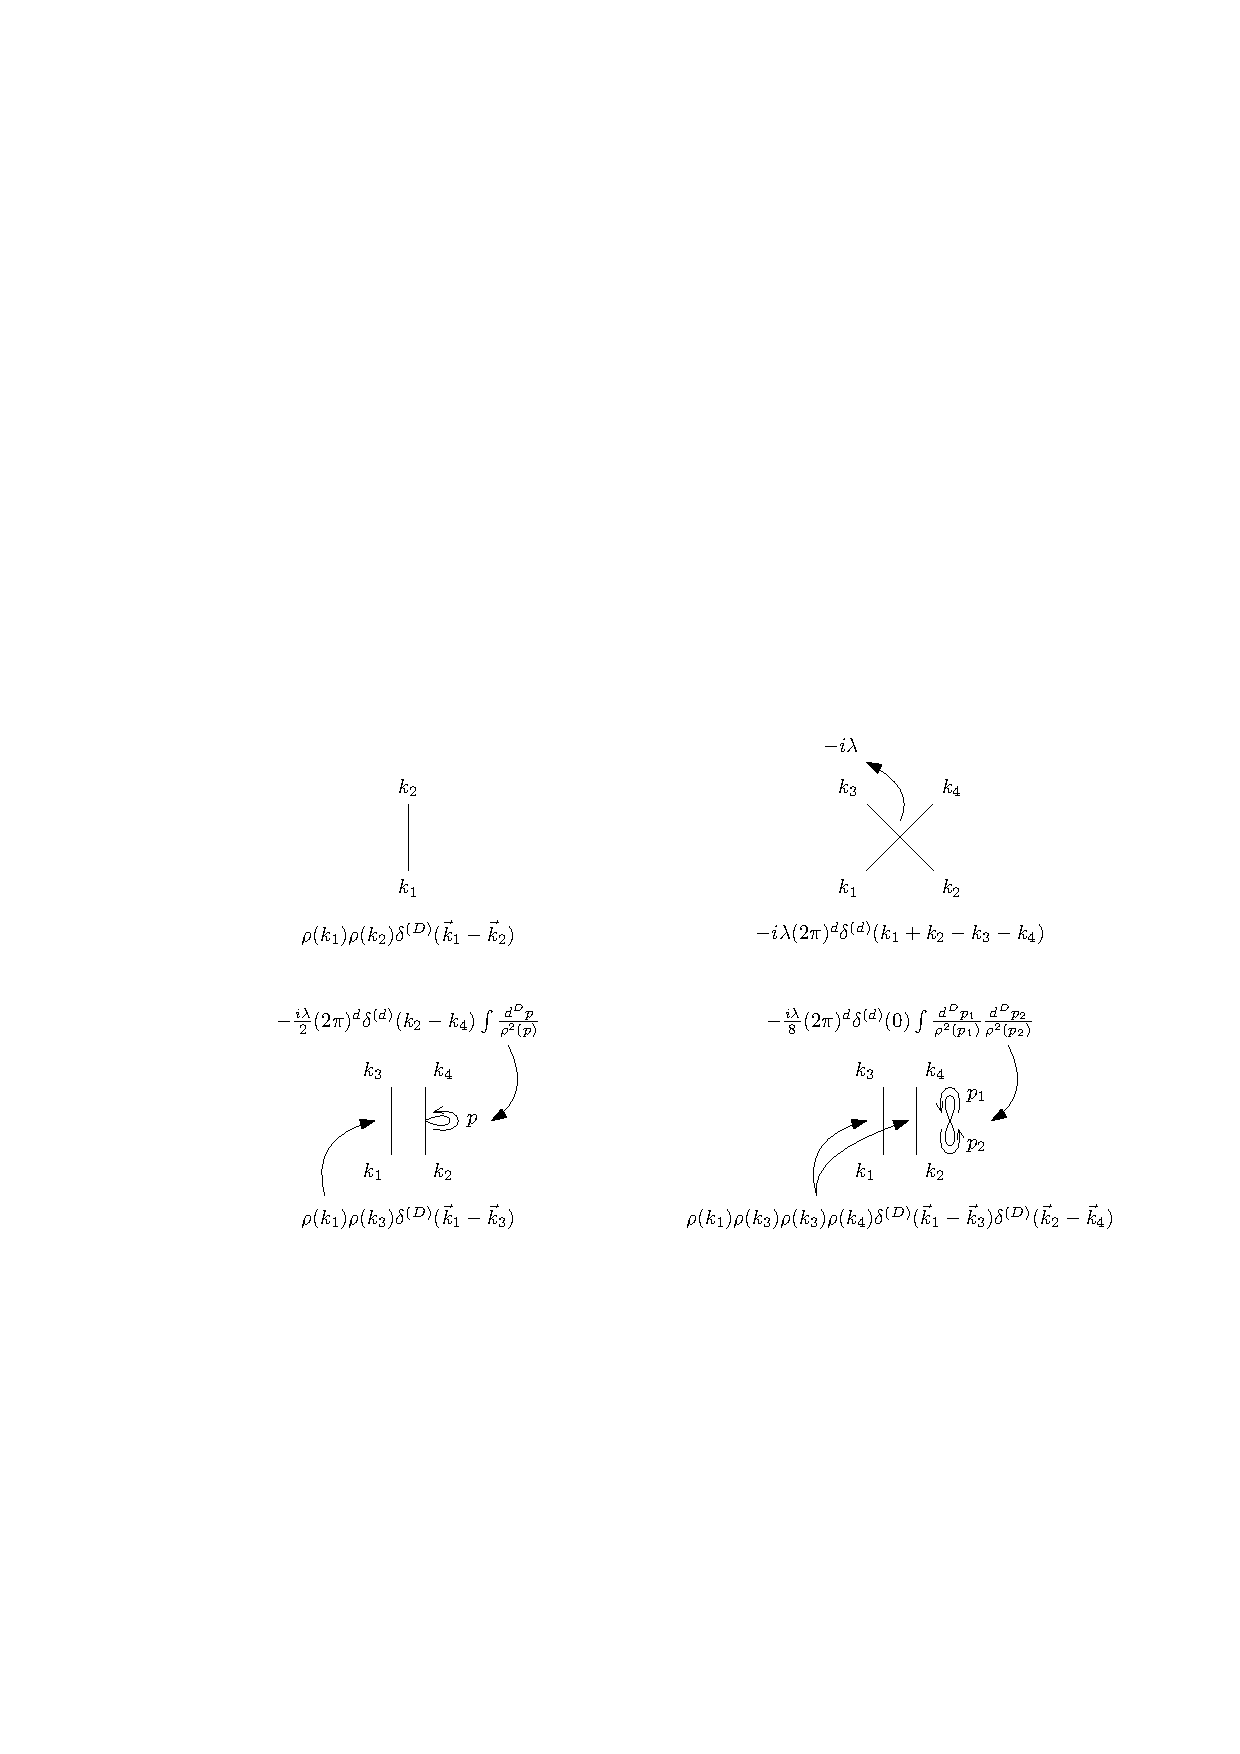
\includegraphics[scale=1]{figures/canonical quantization - Feynman diagrams.pdf}
		\caption{canonical quantization - Feynman diagrams.}
	\end{figure}
	
	观察可见, 上图和 figure \ref{figure Feynman diagrams.3} 有对应关系.
	
	\item 再举一个例子,
	\begin{align}
		& \vcenter{\hbox{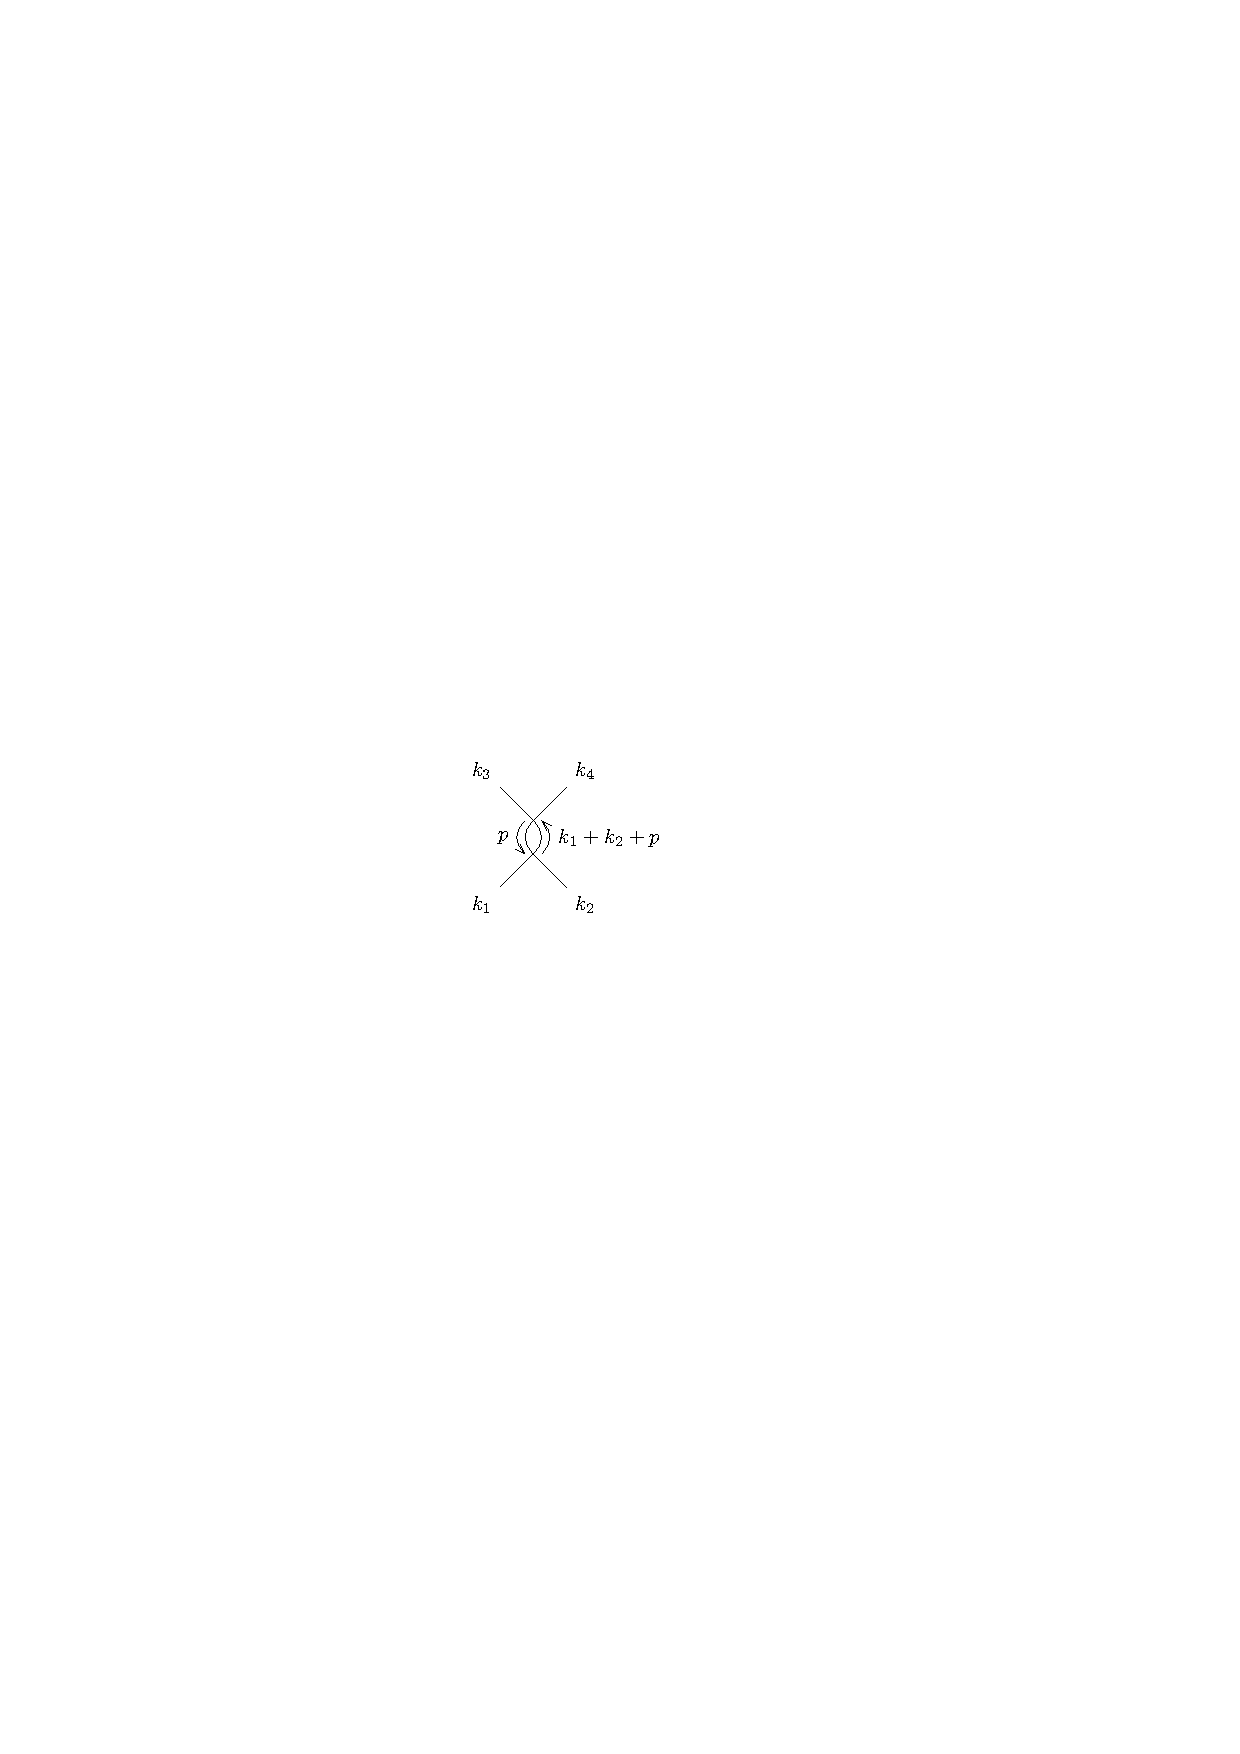
\includegraphics[scale=1]{figures/another loop diagram.pdf}}} \notag \\
		=& (4 \times 3)^2 \times 2 \times \Big( \frac{- i \lambda}{4!} \Big)^2 \rho(k_1) \cdots \int d^d x_1 d^d x_2 \int \frac{d^D p_1 \cdots}{\rho(p_1) \cdots} \frac{d^D q_1 \cdots}{\rho(q_1) \cdots} e^{i (p_1 + p_2 - p_3 - p_4) \cdot x_1} e^{i (q_1 + q_2 - q_3 - q_4) \cdot x_2} \notag \\
		& \Big( \theta(t_2 - t_1) \braket{0 | \wick{
			\c3 a_{\vec{k}_3} \c4 a_{\vec{k}_4} \c5 a_{\vec{q}_1} \c6 a_{\vec{q}_2} \c3 a^\dag_{\vec{q}_3} \c4 a^\dag_{\vec{q}_4} \c1 a_{\vec{p}_1} \c2 a_{\vec{p}_2} \c5 a^\dag_{\vec{p}_3} \c6 a^\dag_{\vec{p}_4} \c1 a^\dag_{\vec{k}_1} \c2 a^\dag_{\vec{k}_2}
		} | 0} + \cdots \Big) \notag \\
		=& \frac{(- i \lambda)^2}{2} \int d^d x_1 d^d x_2 \int \frac{d^D p_3}{\rho^2(p_3)} \frac{d^D p_4}{\rho^2(p_4)} \Big( \theta(t_2 - t_1) e^{i (k_1 + k_2 - p_3 - p_4) \cdot x_1} e^{i (p_3 + p_4 - k_3 - k_4) \cdot x_2} \notag \\
		& + \theta(t_1 - t_2) e^{i (k_1 + k_2 + p_3 + p_4) \cdot x_1} e^{i (- p_3 - p_4 - k_3 - k_4) \cdot x_2} \Big) \notag \\
		=& \frac{(- i \lambda)^2}{2} \int d^d x_1 d^d x_2 \, e^{i ((k_1 + k_2) \cdot x_1 - (k_3 + k_4) \cdot x_2)} \int \frac{d^D p_3}{\rho^2(p_3)} \frac{d^D p_4}{\rho^2(p_4)} \Big( \theta(t_2 - t_1) e^{i (p_3 + p_4) \cdot (x_2 - x_1)} \notag \\
		& + \theta(t_1 - t_2) e^{i (p_3 + p_4) \cdot (x_1 - x_2)} \Big), \label{canonical quantization.3.5}
	\end{align}
	同样, 与 \eqref{Feynman diagrams.3.18} 有对应关系, (注意按时间排序 $\braket{k_3 k_4 | T(\phi^4(x_1) \phi^4(x_2)) | k_1 k_2}$).
	
	\begin{tcolorbox}[title=calculation:]
		从 \eqref{Feynman diagrams.3.17} 开始 (与 \eqref{free field theory.2.1} 类似, $\vec{p}, \vec{q}$ 的符号可以任意改变),
		\begin{align}
			& \int d^d x_1 d^d x_2 \, e^{i (k_1 + k_2 + p - q) \cdot x_1} e^{i (k_3 + k_4 - p + q) \cdot x_2} \int \frac{d^d p}{(2 \pi)^d} \frac{d^d q}{(2 \pi)^d} \frac{i}{- p^2 - m^2 + i \epsilon} \frac{i}{- q^2 - m^2 + i \epsilon} \notag \\
			=& \int d^d x_1 d^d x_2 \, e^{i ((k_1 + k_2) \cdot x_1 + (k_3 + k_4) \cdot x_2)} \int \frac{d^d p}{(2 \pi)^d} \frac{d^d q}{(2 \pi)^d} \frac{i e^{i p \cdot (x_1 - x_2)}}{- p^2 - m^2 + i \epsilon} \frac{i e^{i e^{i q \cdot (x_2 - x_1)}}}{- q^2 - m^2 + i \epsilon} \notag \\
			=& \int d^d x_1 d^d x_2 \, e^{i ((k_1 + k_2) \cdot x_1 + (k_3 + k_4) \cdot x_2)} \int \frac{d^D p}{(2 \pi)^d} \frac{d^D q}{(2 \pi)^d} \Big( \theta(t_2 - t_1) \frac{2 \pi i^2 e^{- i p \cdot (x_1 - x_2)}}{- 2 \omega_p} \notag \\
			& \frac{- 2 \pi i^2 e^{i q \cdot (x_2 - x_1)}}{2 \omega_q} + \theta(t_1 - t_2) \frac{- 2 \pi i^2 e^{i p \cdot (x_1 - x_2)}}{2 \omega_p} \frac{2 \pi i^2 e^{- i q \cdot (x_2 - x_1)}}{- 2 \omega_q} \Big) \notag \\
			=& \int d^d x_1 d^d x_2 \, e^{i ((k_1 + k_2) \cdot x_1 + (k_3 + k_4) \cdot x_2)} \int \frac{d^D p}{\rho^2(p)} \frac{d^D q}{\rho^2(q)} \Big( \theta(t_2 - t_1) e^{i (p + q) \cdot (x_2 - x_1)} \notag \\
			& + \theta(t_1 - t_2) e^{i (p + q) \cdot (x_1 - x_2)} \Big),
		\end{align}
		结果与 \eqref{canonical quantization.3.5} 对应.
	\end{tcolorbox}
\end{itemize}

\section{complex scalar field} \label{canonical quantization.4}
\begin{itemize}
	\item complex scalar field 的 Lagrangian 为
	\begin{equation}
		\mathcal{L} = - (\partial \psi^\dag) (\partial \psi) - m^2 \psi^\dag \psi,
	\end{equation}
	实际上, complex scalar field 可以视为 2 个 real scalar fields 的和
	\begin{equation}
		\psi = \frac{1}{\sqrt{2}} (\phi_1 + i \phi_2) \Longrightarrow \Big| \frac{\partial \phi_1, \phi_2}{\partial \psi, \psi^\dag} \Big| = i,
	\end{equation}
	因此, 也可以把 $\psi, \psi^\dag$ 视为两个独立的场.
	
	\item 其 canonical momentum 为
	\begin{equation}
		\pi(x) = \frac{\delta \mathcal{L}}{\delta \partial_0 \psi} = \partial_0 \psi^\dag, \quad \pi^\dag = \partial_0 \psi,
	\end{equation}
	其 Hamiltonian 为
	\begin{align}
		& \mathcal{H} = \pi^\dag \pi + (\vec{\nabla} \psi^\dag) \cdot (\vec{\nabla} \psi) + m^2 \psi^\dag \psi, \\
		\Longrightarrow & \begin{dcases}
			\partial_0 \pi = i [H, \pi] = \vec{\nabla}^2 \psi^\dag - m^2 \psi^\dag \\
			\partial_0 \psi = i [H, \psi] = \pi^\dag
		\end{dcases} \Longrightarrow (- \partial^2 - m^2) \psi = 0.
	\end{align}
	
	\item 求解得到 (其中 $k^0 = \omega_k$)
	\begin{equation}
		\psi(x) = \int \frac{d^D k}{\rho(k)} (a_{\vec{k}} e^{i k \cdot x} + b^\dag_{\vec{k}} e^{- i k \cdot x}).
	\end{equation}
	
	\noindent\rule[0.5ex]{\linewidth}{0.5pt} % horizontal line
	
	\item 从 path integral 的角度,
	\begin{align}
		Z(J, J^\dag) &= \int D\psi D\psi^\dag \, e^{i \int d^d x \, (\psi^\dag (\partial^2 - m^2) \psi + J^\dag \psi + \psi^\dag J)} \\
		&= \mathcal{C} e^{- \frac{i}{2} \int d^d x d^d y \, 2 J^\dag(x) D(x - y) J(y)}.
	\end{align}
	
	\begin{tcolorbox}[title=calculation:]
		转换为 $\phi_1, \phi_2$ 后计算路径积分,
		\begin{align}
			Z(J, J^\dag) &= \mathcal{C} e^{- \frac{i}{2} \int d^d x d^d y \, (J_1(x) D(x - y) J_1(y) + J_2(x) D(x - y) J_2(y))} \notag \\
			&= \mathcal{C} e^{- \frac{i}{2} \int d^d x d^d y \, 2 J^\dag(x) D(x - y) J(y)}.
		\end{align}
	\end{tcolorbox}
\end{itemize}

\subsection{charge}
\begin{itemize}
	\item 对场算符做如下变换,
	\begin{equation}
		\psi(x, \lambda) = e^{i \lambda} \psi(x) \Longrightarrow D_\lambda \mathcal{L} = 0.
	\end{equation}
	
	\item 因此, 得到 conserved current,
	\begin{equation}
		J^\mu = \pi^\mu D_\lambda \psi + \pi^{\dag \mu} D_\lambda \psi^{\dag} = i (\psi \partial^\mu \psi^\dag - \psi^\dag \partial^\mu \psi),
	\end{equation}
	其 $0$ 分量对空间积分就是 charge,
	\begin{align}
		Q &= \int d^D x \, J^0 = \int d^D x \, i (\psi^\dag \partial_0 \psi - \psi \partial_0 \psi^\dag) \notag \\
		&= \int d^D k \, (a^\dag_{\vec{k}} a_{\vec{k}} - b^\dag_{\vec{k}} b_{\vec{k}}).
	\end{align}
	
	\begin{tcolorbox}[title=calculation:]
		\begin{align}
			Q =& \int d^D x \int \frac{d^D p}{\rho(p)} \frac{d^D q}{\rho(q)} i \Big( (a^\dag_{\vec{p}} e^{- i p \cdot x} + b_{\vec{p}} e^{i p \cdot x}) (- i \omega_q) (a_{\vec{q}} e^{i q \cdot x} - b^\dag_{\vec{q}} e^{- i q \cdot x}) \notag \\
			& - (a_{\vec{q}} e^{i q \cdot x} + b^\dag_{\vec{q}} e^{- i q \cdot x}) (i \omega_p) (a^\dag_{\vec{p}} e^{- i p \cdot x} - b_{\vec{p}} e^{i p \cdot x}) \Big) \notag \\
			=& \int d^D x \int \frac{d^D p}{\rho(p)} \frac{d^D q}{\rho(q)} \Big( (\omega_p a_{\vec{q}} a^\dag_{\vec{p}} + \omega_q a^\dag_{\vec{p}} a_{\vec{q}}) e^{- i (p - q) \cdot x} - (\omega_p b^\dag_{\vec{q}} b_{\vec{p}} + \omega_q b_{\vec{p}} b^\dag_{\vec{q}}) e^{i (p - q) \cdot x} \notag \\
			& + a^\dag_{\vec{p}} b^\dag_{\vec{q}} (\omega_p - \omega_q) e^{- i (p + q) \cdot x} - a_{\vec{q}} b_{\vec{p}} (\omega_p - \omega_q) e^{i (p + q) \cdot x} \Big) \notag \\
			=& \int \frac{d^D p}{\rho(p)} \frac{d^D q}{\rho(q)} \notag \\
			& \Big( \Big( (\omega_p a_{\vec{q}} a^\dag_{\vec{p}} + \omega_q a^\dag_{\vec{p}} a_{\vec{q}}) e^{i (\omega_p - \omega_q) \cdot t} - (\omega_p b^\dag_{\vec{q}} b_{\vec{p}} + \omega_q b_{\vec{p}} b^\dag_{\vec{q}}) e^{- i (\omega_p - \omega_q) \cdot t} \Big) (2 \pi)^D \delta^{(D)}(\vec{p} - \vec{q}) \notag \\
			& + \Big( a^\dag_{\vec{p}} b^\dag_{\vec{q}} (\omega_p - \omega_q) e^{i (\omega_p + \omega_q) \cdot x} - a_{\vec{q}} b_{\vec{p}} (\omega_p - \omega_q) e^{- i (\omega_p + \omega_q) \cdot x} \Big) (2 \pi)^D \delta^{(D)}(\vec{p} + \vec{q}) \Big) \notag \\
			=& \int \frac{d^D k}{2} \, (a_{\vec{k}} a^\dag_{\vec{k}} + a^\dag_{\vec{k}} a_{\vec{k}} - b_{\vec{k}} b^\dag_{\vec{k}} - b^\dag_{\vec{k}} b_{\vec{k}}) = \int d^D k \, (a^\dag_{\vec{k}} a_{\vec{k}} - b^\dag_{\vec{k}} b_{\vec{k}}).
		\end{align}
	\end{tcolorbox}
	
	\item 代入 \eqref{classical field theory and Noether's theorem.3.2}, 有 $i [Q, \psi] = - i \psi$, 所以
	\begin{equation}
		e^{- i \lambda Q} \psi e^{i \lambda Q} = e^{i \lambda} \psi.
	\end{equation}
\end{itemize}
